\begin{frame}[plain,c]
\begin{center}
{\Huge \bf Optional reading for Lecture \thislecture}
\end{center}
\end{frame}

% ------------------------------------------------------------------------------

%
% Worked example :
%

{
\problemslide

%
%
%

\begin{frame}{Worked example: Wire falling in magnetic field}

  \begin{blockexmplque}{Question}
    \begin{minipage}[l]{0.22\textwidth}
     \begin{center}
         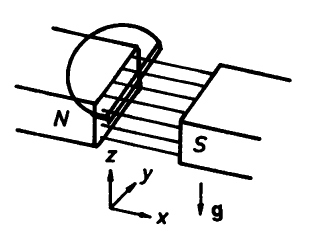
\includegraphics[width=0.90\textwidth]{./images/problems/lect08_wire_falls_in_b_field}
     \end{center}
    \end{minipage}
    \begin{minipage}[r]{0.75\textwidth}
       A long straight wire parallel to the $y$ axis lies in a uniform magnetic
       field $\vec{B} = B \hat{x}$, as shown in the figure on the left.
       The mass per unit length and resistance per unit length of the wire
       are $\lambda_{m}$ and $\lambda_{r}$ respectively.\\
    \end{minipage}
    \vspace{0.1cm}
    The wire may be considered to extend to the edges of the field,
    where the ends are connected to one another by a massless perfect conductor
    which lies outside the field. Fringing effects can be neglected.\\
    The wire is allowed to fall under the influence of gravity $(\vec{g} = -g \hat{z})$.\\
    Find:
    \begin{itemize}
    \item the electromotive force developed across the wire,
    \item the current flowing along the wire,
    \item the magnetic force acting on the wire, and
    \item the terminal velocity of the wire as it falls through the magnetic field.
    \end{itemize}
  \end{blockexmplque}

\end{frame}

%
%
%

\begin{frame}{Worked example: Wire falling in magnetic field}

  As the wire falls within the magnetic field with a velocity $u$,
  the EMF $\varepsilon$ developed across the wire is given by:
  \begin{equation*}
    \varepsilon = \int (\vec{u} \times \vec{B}) \cdot d\vec{\ell}
                = uB\ell
  \end{equation*}
  where $\ell$ is the length of the wire
  (which is fully within the magnetic field).

  The resistance $R$ of the wire of length $\ell$ is:
  \begin{equation*}
    R = \lambda_{r} \ell
  \end{equation*}

  Therefore, the current that will flow in the wire is given by:
  \begin{equation*}
    I = \frac{\varepsilon}{R}
      = \frac{uB\cancel{\ell}}{\lambda_{r}\cancel{\ell}}
      = \frac{uB}{\lambda_{r}}
  \end{equation*}
  This current is flowing towards the $-\hat{y}$ direction.

\end{frame}

%
%
%

\begin{frame}{Worked example: Wire falling in magnetic field}

  The force exerted on the current-carrying wire because of the
  magnetic field is:
  \begin{equation*}
    \vec{F}_{B} =
     I \int d\vec{\ell} \times \vec{B}
  \end{equation*}

  Substituting $I$ from the previous expression, and considering
  $d\vec{\ell}$ to be in the direction of the current, we have:
  \begin{equation*}
    \vec{F}_{B} =
     \frac{uB}{\lambda_{r}} \int \Big( dy(-\hat{y})\Big) \times \Big( B \hat{x}\Big) =
     \frac{uB^2}{\lambda_{r}} \Big(\int dy \Big) \Big(- \hat{y}) \times \hat{x}\Big) \Rightarrow
  \end{equation*}
  \begin{equation*}
    \vec{F}_{B} =
     \frac{uB^2\ell}{\lambda_{r}} \hat{z}
  \end{equation*}
  This force will oppose the downwards gravitational force $\vec{F}_{g}$.

\end{frame}

%
%
%

\begin{frame}{Worked example: Wire falling in magnetic field}

  The wire carries a mass given by:
  \begin{equation*}
     m = \lambda_{m} \ell
  \end{equation*}
  and, therefore, the force of gravity is:
  \begin{equation*}
     \vec{F}_{g} = m \vec{g} = - \lambda_{m} \ell g \hat{z}
  \end{equation*}

  The wire will reach its terminal velocity $u^{\prime}$ when the
  two forces cancel each other out exactly.
  Therefore, $u^{\prime}$ is given by the condition:
  \begin{equation*}
     \frac{u^{\prime} B^2 \cancel{\ell}}{\lambda_{r}} = \lambda_{m} \cancel{\ell} g
  \end{equation*}

  Solving for $u^{\prime}$ we find:
  \begin{equation*}
     u^{\prime} = \frac{\lambda_{r} \lambda_{m} g}{B^2}
  \end{equation*}

\end{frame}

} % Worked example

% ------------------------------------------------------------------------------

%
% Worked example :
%

{
\problemslide

%
%
%

\begin{frame}{Worked example: Displacement current in capacitor}

  \begin{blockexmplque}{Question}
    At what rate must the potential difference between the plates
    of a parallel plate capacitor with a 2.0 $\mu$F capacitance
    be changed to produce a displacement current of 1.5 A?
  \end{blockexmplque}

  Let the area plate be A and the plate separation be d.
  The displacement current $I_{d}$ is:

  \begin{equation*}
    I_{d} = \epsilon_0 \frac{d\Phi_{E}}{dt}
    \xRightarrow{\Phi_{E} = EA}
    I_{d} = \epsilon_0 \frac{d}{dt} (EA)
          = \epsilon_0 A \frac{dE}{dt}
  \end{equation*}

  \begin{equation*}
    \xRightarrow{E = V/d}
    I_{d} = \epsilon_0 A \frac{d}{dt} (\frac{V}{d})
          = \frac{\epsilon_0 A}{d} \frac{dV}{dt}
    \xRightarrow{C = \epsilon_0 A/d}
    I_{d} = C \frac{dV}{dt}
  \end{equation*}

  \begin{equation*}
    \Rightarrow
     \frac{dV}{dt} = \frac{I_{d}}{C}
                   = \frac{15.0 \; A}{2 \times 10^{-6} \; F}
                   = 7.5 \times 10^{5} \; V/s
  \end{equation*}

\end{frame}

} % Worked example

% ------------------------------------------------------------------------------

%
% Worked example :
%

{
\problemslide

%
%
%

\begin{frame}{Worked example: Induced current in rectangular wire loop}

  \begin{blockexmplque}{Question}

    The figure below shows a wire that forms a rectangle (W = 20 cm, H = 30 cm)
    and has a resistance of 5.0 m$\Omega$. Its interior is split into three
    equal areas, with magnetic fields $\vec{B}_{1}$, $\vec{B}_{2}$ and $\vec{B}_{3}$.
    The fields are uniform within each region and directly
    out of or into the page as indicated.

    The graph below gives the change in the z components (B$_{z}$)
    of the three fields with time t;
    the vertical axis scale is set by
    B$_{s}$ = 4.0 $\mu$T and B$_{b}$ = 2.5B$_{s}$
    and the horizontal axis scale is set by t$_{s}$ = 2.0 s.

    \begin{minipage}[r]{0.30\textwidth}
      What are the
      \begin{itemize}
        \item magnitude, and
        \item direction of the current induced in the wire?
      \end{itemize}
    \end{minipage}
    \begin{minipage}[l]{0.30\textwidth}
     \begin{center}
    	 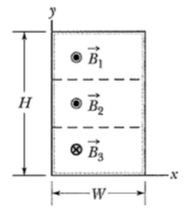
\includegraphics[width=0.95\textwidth]{./images/problems/lect08_rectangular_wire_3bfield_regions}\\
     \end{center}
    \end{minipage}
    \begin{minipage}[l]{0.38\textwidth}
     \begin{center}
    	 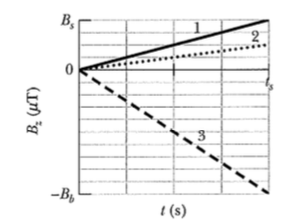
\includegraphics[width=0.95\textwidth]{./images/problems/lect08_rectangular_wire_3bfield_regions_Bz}\\
     \end{center}
    \end{minipage}

  \end{blockexmplque}

\end{frame}

%
%
%

\begin{frame}{Worked example: Induced current in rectangular wire loop}

  \vspace{-0.2cm}

  The induced emf is:
  \begin{equation*}
     \varepsilon = - \sum_{i} \frac{d\Phi_{B;i}}{dt}
  \end{equation*}

  If the surface vector of the loop is collinear with
  $\vec{B}_1$ and $\vec{B}_2$, the flux due to $\vec{B}_1$ and $\vec{B}_2$
  is positive, whereas the flux due to $\vec{B}_3$ is negative. Therefore:
  \begin{equation*}
     \varepsilon = \frac{1}{3} H W
      \Big\{ - \frac{dB_1}{dt} - \frac{dB_2}{dt} + \frac{dB_3}{dt} \Big\} =
  \end{equation*}
  \begin{equation*}
     \frac{(0.30 \; m) (0.20 \; m)}{3}
                     \Big\{ - \frac{4  \times 10^{-6} \; T}{2.0 \; s}
                            - \frac{2  \times 10^{-6} \; T}{2.0 \; s}
                            + \frac{10 \times 10^{-6} \; T}{2.0 \; s} \Big\}
     = 4 \times 10^{-8} \; V
  \end{equation*}

  The plus sign means that the emf is dominated by changes in $\vec{B}_3$.

  The current induced by $\varepsilon$ is:
  \begin{equation*}
    I = \frac{|\varepsilon|}{R} = \frac{4 \times 10^{-8} \; V}{5 \times 10^{-3} \; \Omega}
      \approx 8 \; {\mu}A
  \end{equation*}

  By Lenz's law, the induced emf (and current) resist to these changes in the magnetic flux.
  Therefore, the direction of the current is counter-clockwise.

\end{frame}

} % Worked example

% ------------------------------------------------------------------------------

%
% Worked example :
%

{
\problemslide

%
%
%

\begin{frame}{Worked example: Loop in uniform time-dependent $\vec{B}$}

  \begin{blockexmplque}{Question}

    \begin{minipage}[l]{0.30\textwidth}
     \begin{center}
    	 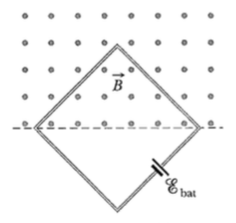
\includegraphics[width=0.98\textwidth]{./images/problems/lect08_square_loop_with_emf_partially_within_bfield}\\
     \end{center}
    \end{minipage}
    \begin{minipage}[r]{0.69\textwidth}
      A square wire loop with 2.00 m sides is perpendicular to a uniform
      magnetic field, with half the area of the loop in the field,
       as shown in the figure on the left.

      The loop contains an ideal battery with emf $\varepsilon_{bat}$ = 20 V.
      If the magnitude of the field varies with time according
      to $B$ = 0.0420 - 0.870$t$,
      with $B$ in Teslas and $t$ in seconds, what are the
      \begin{itemize}
        \item net emf in the circuit, and
        \item the direction of the (net) emf around the loop?
      \end{itemize}
    \end{minipage}

  \end{blockexmplque}

  Let $L$ be the length of a side of the square circuit.
  Then the magnetic flux through the circuit is:
  \begin{equation*}
    \Phi_B = \frac{1}{2} L^2 B
  \end{equation*}

\end{frame}

%
%
%

\begin{frame}{Worked example: Loop in uniform time-dependent $\vec{B}$}

  The induced emf is:
  \begin{equation*}
    \varepsilon_{induced} = - \frac{d\Phi_{B}}{dt} = - \frac{1}{2} L^2 \frac{dB}{dt}
  \end{equation*}

  The rate of change of the given field is:
  \begin{equation*}
    \frac{dB}{dt} = \frac{d}{dt} (0.0420 - 0.870t) = -0.870 \; T/s
  \end{equation*}

  Therefore, the induced emf is:
  \begin{equation*}
    \varepsilon_{induced} = - \frac{1}{2} (2.0 \; m)^2 (-0.870 \; T/s) = 1.74 \; V
  \end{equation*}

  The magnetic field is out of the page and decreasing so the induced emf is
  counterclockwise around the circuit, in the same direction
  as the emf of the battery. The total emf is:
  \begin{equation*}
    \varepsilon_{total} =
      \varepsilon_{induced} + \varepsilon_{battery} = 1.74 \; V + 20 \; V = 21.74 \; V
  \end{equation*}

\end{frame}

} % Worked example

% ------------------------------------------------------------------------------

%
% Worked example :
%

{
\problemslide

%
%
%

\begin{frame}{Worked example: Loop in non-uniform time-dependent $\vec{B}$}

  \begin{blockexmplque}{Question}

  \begin{minipage}[l]{0.34\textwidth}
   \begin{center}
  	 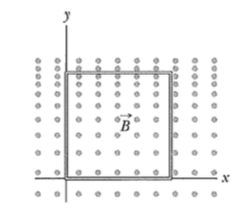
\includegraphics[width=0.88\textwidth]{./images/problems/lect08_square_loop_in_nonuniform_bfield}\\
   \end{center}
  \end{minipage}
  \begin{minipage}[r]{0.65\textwidth}
    As seen in the figure on the left, a square loop of wire has sides of
    length 2.0 cm. A magnetic field is directed out of the page; its magnitude
    is given by $B$ = 4.0$t^2$$y$, where $B$ is in Teslas, $t$ is in seconds,
    and $y$ is in meters.
    At $t$ = 2.5 s, what are the
    \begin{itemize}
      \item magnitude, and
      \item direction of the emf induced in the loop?
    \end{itemize}
  \end{minipage}

  \end{blockexmplque}

  Consider a (thin) strip of area of height $dy$ and width $\ell$ = 0.020 m.
  The strip is located at position $y$ (0 $<$ $y$ $<$ $\ell$).
  The magnetic field in that thin strip is uniform and, therefore,
  the magnetic flux through that strip is:
  \begin{equation*}
     d\Phi_{B} = B dA = (4 t^2 y)(\ell dy)
  \end{equation*}

\end{frame}

%
%
%

\begin{frame}{Worked example: Loop in non-uniform time-dependent $\vec{B}$}

  The total flux through the square loop is:
  \begin{equation*}
     \Phi_{B} = \int d\Phi_{B} = \int_{0}^{\ell} 4 t^2 y \ell dy
              = 4 t^2 \ell \int_{0}^{\ell} y dy
              = 2 t^2 \ell^3
  \end{equation*}
  Thus, Faraday's law yields:
  \begin{equation*}
    \varepsilon = - \frac{d\Phi_{B}}{dt} = - 4 t \ell^3
  \end{equation*}
  At $t$ = 2.5 s, the magnitude of the emf is:
  \begin{equation*}
    |\varepsilon| = 4 (2.5 \; s) (0.02 \; m)^3 = 8.0 \times 10^{-5} \; V
  \end{equation*}

  The emf direction is clockwise, by Lenz's law.

\end{frame}

} % Worked example

% ------------------------------------------------------------------------------

%
% Worked example :
%

{
\problemslide

%
%
%

\begin{frame}{Worked example: Charging a parallel-plate capacitor}

  \begin{blockexmplque}{Question}

    A parallel-plate capacitor has square plates of edge length $L$ = 1.0 m.
    A current of 2.0 A charges the capacitor, producing a uniform electric
    field $\vec{E}$ between the plates, with $\vec{E}$ perpendicular to the plates.\\
    \vspace{0.2cm}
    \begin{minipage}[l]{0.19\textwidth}
     \begin{center}
    	 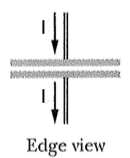
\includegraphics[width=0.98\textwidth]{./images/problems/lect08_parallel_plate_capacitor_edge_view}\\
     \end{center}
    \end{minipage}
    \begin{minipage}[l]{0.19\textwidth}
     \begin{center}
    	 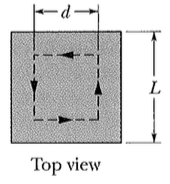
\includegraphics[width=0.98\textwidth]{./images/problems/lect08_parallel_plate_capacitor_top_view}\\
     \end{center}
    \end{minipage}
    \begin{minipage}[r]{0.60\textwidth}
      \begin{itemize}
        \item What is the displacement current $I_{d}$
          through the region between the plates?
        \item What is $dE/dt$ in this region?
        \item What is the displacement current encircled
          by the square dashed path of edge length $d$ = 0.50 m?
        \item What is $\oint \vec{B} \cdot d\vec{\ell}$
          around this square dashed path?
      \end{itemize}
    \end{minipage}

  \end{blockexmplque}

\end{frame}

%
%
%

\begin{frame}{Worked example: Charging a parallel-plate capacitor}

  As the current $I$ charges the capacitor, the electric field between
  the plates of the capacitor is changing.
  This produces a displacement current $I_{d}$ bet- ween the plates,
  which is given by:
  \begin{equation*}
    I_d = \epsilon_0 \frac{d\Phi_{E}}{dt}
  \end{equation*}

  Let $A$ be the area of a plate, $d$ the plate separation,
  and $E$ the magnitude of the electric field between the plates.
  $E$ is uniform, and it is given by:
  \begin{equation*}
    E = \frac{V}{d}
  \end{equation*}
  where $V$ is the potential difference across the plates.

  The current into the positive plate of the capacitor is
  \begin{equation*}
    I = \frac{dQ}{dt} = \frac{d}{dt}(CV) = C \frac{dV}{dt}
      = \frac{\epsilon_0 A}{d} \frac{d(Ed)}{dt}
      = \epsilon_0 A \frac{dE}{dt} = \epsilon_0 \frac{d\Phi_{E}}{dt} = I_{d}
  \end{equation*}

  At any time, the conduction current $I$ in the wires equals
  the displacement current $I_{d}$ in the gap between the plates,
  and thus $I_{d}$ = 2.0 A.

\end{frame}

%
%
%

\begin{frame}{Worked example: Charging a parallel-plate capacitor}

  The rate of change of the electic field is:
  \begin{equation*}
    I_d = \epsilon_0 A \frac{dE}{dt} \Rightarrow
    \frac{dE}{dt} = \frac{I_d}{\epsilon_0 A} \Rightarrow
  \end{equation*}
  \begin{equation*}
    \frac{dE}{dt} = \frac{2.0 \; A}{(8.85 \times 10^{-12} \; F/m)(1.0 \; m^2)}
                  = 2/3 \times 10^{11} \frac{V}{m \cdot s}
  \end{equation*}

  The displacement current $I_d^\prime$ through the indicated path is
  \begin{equation*}
    I_d^\prime = I_d \frac{d^2}{L^2}
               = (2.0 \; A) \frac{(0.5 \; m)^2}{(1.0 \; m)^2}
               = (2.0 \; A) \frac{1}{4} = 0.5 \; A
  \end{equation*}

   From Ampere's law, the integral of the magnetic field around the indicated path is
   \begin{equation*}
      \oint \vec{B} \cdot d\vec{\ell}
         = \mu_0 I_d^\prime
         = (1.26 \times 10^{-6} \; T \cdot m / A) (0.5 \; A)
         = 6.3 \times 10^{-7} \; T \cdot m
   \end{equation*}

\end{frame}

} % Worked example

% ------------------------------------------------------------------------------

%
% Worked example :
%

{
\problemslide

%
%
%

\begin{frame}{Worked example: Charging a parallel-plate capacitor 2}

  \begin{blockexmplque}{Question}
    A parallel-plate capacitor with circular plates is being charged.
    Consider a circular loop centred on the central axis and located between
    the plates. If the loop radius of 3 cm is greater than the plate radius,
    what is the displacement current between the plates when the magnetic
    field along the loop has magnitude 2 $\mu$T?
  \end{blockexmplque}

  From Ampere's law, the line integral of $\vec{B}$ along the
  circular loop $L$ is
  \begin{equation*}
    \oint_{L} \vec{B} \cdot d\vec{\ell} = \mu_0 (I + I_D)
  \end{equation*}
  where $I$ ($I_D$) is the conduction (displacement)
  current through a surface that has the
  circular loop $L$ as its boundary.

\end{frame}

%
%
%

\begin{frame}{Worked example: Charging a parallel-plate capacitor 2}

  Between the capacitor plates, $I=0$.

  Therefore:
  \begin{equation*}
    I_D = \frac{1}{\mu_0} \oint_{L} \vec{B} \cdot d\vec{\ell}
  \end{equation*}

  From the cylindrical symmetry of the problem ($B$ is constant along $L$,
  and $\vec{B}$ is parallel to $d\vec{\ell}$), we find:
  \begin{equation*}
    \oint_{L} \vec{B} \cdot d\vec{\ell} = 2\pi r B
  \end{equation*}

  Finally:
  \begin{equation*}
    I_D = \frac{2\pi r B}{\mu_0} \Rightarrow
  \end{equation*}
  \begin{equation*}
    I_D =
      \frac{2\pi(0.03\;m)(2 \times 10^{-6} \; T)}{4\pi \times 10^{-7}\; Tm/A} =
      0.3 \; A
  \end{equation*}

\end{frame}

} % Worked example
% ------------------------------------------------------------------------------
